%% ============================================================
%% ACM MM Workshop 2026 — Submission-ready file
%% Compiler : pdfLaTeX  (set in Overleaf → Menu → Compiler)
%% Template : ACM Conference Proceedings  (acmart sigconf)
%% ============================================================
\documentclass[sigconf,nonacm]{acmart}

%% ── Safe packages (do NOT add subcaption / hyperref / xcolor;
%%    acmart loads them internally and will throw option clashes) ──
\usepackage{booktabs}
\usepackage{multirow}
\usepackage{amsmath}
%% amssymb removed — acmart loads AMS fonts via newtxmath; double-loading
%% causes the "\Bbbk already defined" compile error.
\usepackage{microtype}
\usepackage{graphicx}

%% Suppress ACM copyright / rights block
\settopmatter{printacmref=false, printfolios=true}
\renewcommand\footnotetextcopyrightpermission[1]{}

%% ── Title ────────────────────────────────────────────────────
\title[VideoMAE-B for Violence Detection]{%
Frozen VideoMAE-B Representations for
Weakly-Supervised Violence Detection and Temporal Localization}

%% ── Single author ────────────────────────────────────────────
\author{Srinivasa Sai Chava}
\affiliation{%
  \institution{Boston University}
  \city{Boston}
  \state{Massachusetts}
  \country{USA}}
\email{saichava@bu.edu}

%% ── Abstract ─────────────────────────────────────────────────
\begin{abstract}
Weakly-supervised video anomaly detection (VAD) has relied on
two-stream I3D features for half a decade despite dramatic advances
in video representation learning.
We present a controlled study of replacing frozen I3D features with
frozen \textbf{VideoMAE-B} features—a masked-autoencoder Vision Transformer
pre-trained on Kinetics-400—within an RTFM + Temporal Refinement Network
(TRN) + Boundary Head framework for surveillance violence detection.
Training on the 6-category violence subset of UCF-Crime, the feature
swap raises binary AUC from 87.4\% to $92.2 \pm 1.3$\% and binary AP
from 82.1\% to $88.7 \pm 1.8$\%.
Temporal localization improves dramatically: mAP@tIoU\,0.3 rises from
0.9\% to $5.8 \pm 1.2$\% (${\times}6.4$), and mAP@0.7 from 0.1\% to
$2.2 \pm 1.0$\% (${\times}21.7$)—the largest gains at strict overlap
thresholds, suggesting that richer spatiotemporal representations produce
sharper event boundaries.
We also contribute a training recipe—inverse-frequency class weights,
confidence-thresholded pseudo-labels, and cosine annealing LR—that
tightens cross-seed variance.
All results are reported over 3 random seeds with mean\,$\pm$\,std.
Code and extracted features will be released upon acceptance.
\end{abstract}

\begin{CCSXML}
<ccs2012>
 <concept>
  <concept_id>10010147.10010178.10010224.10010245.10010251</concept_id>
  <concept_desc>Computing methodologies~Activity recognition and understanding</concept_desc>
  <concept_significance>500</concept_significance>
 </concept>
 <concept>
  <concept_id>10010147.10010178.10010224.10010245.10010246</concept_id>
  <concept_desc>Computing methodologies~Video segmentation</concept_desc>
  <concept_significance>300</concept_significance>
 </concept>
</ccs2012>
\end{CCSXML}

\ccsdesc[500]{Computing methodologies~Activity recognition and understanding}
\ccsdesc[300]{Computing methodologies~Video segmentation}

\keywords{video anomaly detection, violence detection, temporal localization,
          weakly supervised learning, VideoMAE, masked autoencoders}

%% ============================================================
\begin{document}

%% Short author string shown in running header (even pages)
\renewcommand{\shortauthors}{S.~S.~Chava}

\maketitle

%% Plain style: page numbers only, no running headers
%% Must come AFTER \maketitle — acmart resets page style at \maketitle
\pagestyle{plain}
%% ============================================================


%% ============================================================
\section{Introduction}
%% ============================================================

Violence detection in public surveillance is one of the highest-priority
tasks in automated security systems: early alerts for fighting, shooting,
explosion, robbery, and abuse events can dramatically reduce response
latency.
Weakly-supervised video anomaly detection (VAD) addresses this challenge
by learning from video-level binary labels alone—no expensive frame-level
annotation is required.

The dominant paradigm, established by Sultani~et~al.~\cite{sultani2018real}
and refined by RTFM~\cite{tian2021weakly}, extracts segment-level features
from a \emph{frozen} two-stream I3D model pre-trained on
Kinetics-400~\cite{carreira2017quo}, then trains a lightweight Multiple
Instance Learning (MIL) scorer on top.
Despite significant architectural improvements—temporal refinement
modules~\cite{wu2023surveillance}, magnitude-based
learning~\cite{tian2021weakly}, category-aware
routing~\cite{wang2025gsmoe}—\textbf{the feature backbone has remained
largely fixed at I3D since 2017}.

Meanwhile, video foundation models have advanced substantially.
VideoMAE~\cite{tong2022videomae} applies masked autoencoding to video with
a Vision Transformer backbone, learning rich spatiotemporal representations
that substantially outperform I3D on action recognition benchmarks.
A natural question arises: \emph{Does substituting VideoMAE-B for I3D,
with all other components held equal, improve weakly-supervised violence
detection?}

We answer this question affirmatively with controlled experiments on
the UCF-Crime violence subset.
Our contributions are:

\begin{enumerate}
  \item \textbf{VideoMAE-B integration.}
        We extract and cache 16-frame segment features ($D{=}768$) from a
        frozen VideoMAE-B backbone for all 1{,}300 UCF-Crime violence-subset
        videos and demonstrate that this single change yields consistent,
        large improvements across all detection and localization metrics.

  \item \textbf{Violence-aware training recipe.}
        We introduce three complementary training improvements—inverse-frequency
        class weighting, confidence-thresholded pseudo-label filtering, and
        cosine annealing LR—that collectively reduce cross-seed variance without
        modifying the model architecture.

  \item \textbf{Multi-seed reproducibility study.}
        All results are reported over 3 independent random seeds (42, 123, 456)
        with mean\,$\pm$\,std, enabling reliable statistical comparison with
        future work.
\end{enumerate}


%% ============================================================
\section{Related Work}
%% ============================================================

\subsection{Weakly-Supervised Video Anomaly Detection}

Sultani~et~al.~\cite{sultani2018real} formulated VAD as a MIL ranking
problem using anomalous/normal video pairs and C3D features on UCF-Crime.
RTFM~\cite{tian2021weakly} replaced C3D with I3D and added a feature-magnitude
learning module, reaching 84.3\% AUC.
MGFN~\cite{chen2023mgfn} improved to 86.7\% with graph-guided feature
normalization; VadCLIP~\cite{wu2024vadclip} exploited CLIP text-visual
alignment to reach 88.0\%.
Recent work addresses noisy pseudo-labels~\cite{lan2025dss,wang2025dakd},
event completeness~\cite{tian2025lecvad}, and category-specific expert
routing~\cite{wang2025gsmoe}.
\emph{All of these methods continue to use I3D as the video backbone.}
Ours is the first systematic study of replacing I3D with a
masked-autoencoder foundation model in this pipeline.

\subsection{Video Foundation Models}

VideoMAE~\cite{tong2022videomae} extends masked image modeling to video
by masking 90\% of video patches and reconstructing pixel values,
pre-training a ViT-B backbone on Kinetics-400.
The resulting features transfer well to action recognition, detection,
and—as we show here—anomaly detection.
InternVideo~\cite{wang2022internvideo} and
Video-ChatGPT~\cite{maaz2023videochatgpt} further demonstrate the breadth
of video foundation model features across diverse downstream tasks.

\subsection{Violence Detection and Temporal Localization}

XD-Violence~\cite{wu2020not} provided a large-scale multi-modal violence
dataset and showed that audio-visual fusion outperforms vision-only methods.
ActionFormer~\cite{zhang2022actionformer} and TriDet~\cite{shi2023tridet}
achieve strong temporal localization under full supervision but require
expensive frame-level labels.
Our boundary head bridges this gap in the weak-supervision setting.


%% ============================================================
\section{Methodology}
%% ============================================================

Our pipeline follows a \emph{decoupled representation and reasoning} design:
the video backbone is always frozen, and all learnable modules operate on
pre-cached segment features.
Figure~\ref{fig:system} gives an overview of the three-stage pipeline.
Table~\ref{tab:params} summarises architecture components and parameter counts.

\begin{figure*}[t]
  \centering
  
\includegraphics[width=\linewidth]{figures/system_design.png}
  \Description{Three-stage system design. Stage 1: Feature Extraction using
    frozen VideoMAE-B backbone on UCF-Crime videos. Stage 2: Model Architecture
    with MIL Anomaly Scorer, Event Classifier, TRN, and Boundary Head.
    Stage 3: Inference and Evaluation reporting binary AUC, AP, and
    temporal mAP at tIoU 0.3/0.5/0.7.}
  \caption{System design overview.
    \textbf{(1) Feature Extraction}: untrimmed video is split into 16-frame
    segments and encoded by a \emph{frozen} VideoMAE-B backbone, producing
    768-d segment features that are cached to disk.
    \textbf{(2) Model Architecture}: a four-head stack---MIL Anomaly Scorer,
    Event Classifier, Temporal Refinement Network (TRN), and Boundary
    Head---processes the cached features end-to-end with 1.9M trainable
    parameters.
    \textbf{(3) Evaluation}: anomaly scores and boundary predictions are
    thresholded to produce binary AUC/AP and temporal mAP metrics.}
  \label{fig:system}
\end{figure*}

\begin{table}[t]
  \centering
  \caption{Model components and trainable parameter budget.}
  \label{tab:params}
  \small
  \begin{tabular}{lrr}
    \toprule
    \textbf{Component}      & \textbf{Params} & \textbf{Trainable?} \\
    \midrule
    VideoMAE-B backbone     & 86\,M           & No (frozen)         \\
    MIL Scorer              &  1.1\,M         & Yes                 \\
    Event Classifier        &  0.3\,M         & Yes                 \\
    TRN Module              &  0.4\,M         & Yes                 \\
    Boundary Head           &  0.1\,M         & Yes                 \\
    \midrule
    \textbf{Total Trainable} & \textbf{1.9\,M} &                   \\
    \bottomrule
  \end{tabular}
\end{table}

\subsection{Feature Extraction}

Given an untrimmed video $V$, we partition it into non-overlapping 16-frame
segments $\{v_1,\ldots,v_T\}$ (tail segment dropped if $<$16 frames).
Each segment passes through a frozen VideoMAE-B
backbone~\cite{tong2022videomae}\footnote{HuggingFace checkpoint:
\texttt{MCG-NJU/videomae-base-finetuned-kinetics}}:
\begin{equation}
  f_t \;=\; \mathrm{VideoMAE\text{-}B}_{\mathrm{frozen}}(v_t)
       \;\in\; \mathbb{R}^{768}.
\end{equation}
Features are cached as \texttt{.npz} files for all training runs.
By contrast, I3D produces $f_t\in\mathbb{R}^{2048}$; the dimension reduction
from 2{,}048 to 768 also reduces overfitting risk given our dataset size.

\subsection{MIL Anomaly Scorer (RTFM)}

Following RTFM~\cite{tian2021weakly}, a two-layer MLP maps each feature
to an anomaly score:
\begin{equation}
  s_t \;=\; \sigma\!\bigl(W_3\,
            \mathrm{Dropout}\bigl(\mathrm{ReLU}(W_2\,\mathrm{ReLU}(W_1 f_t))\bigr)
            \bigr).
\end{equation}
Video-level score $s_\mathrm{video}=\max_t s_t$.
The MIL ranking loss pairs an anomalous video $a$ with a normal video $n$:
\begin{equation}
  \mathcal{L}_\mathrm{MIL} \;=\;
    \max\!\bigl(0,\;1 - s^{(a)}_\mathrm{video} + s^{(n)}_\mathrm{video}\bigr).
\end{equation}

\subsection{Event Classification Branch}

For each anomalous video with category label $c\in\{1,\ldots,6\}$,
pseudo-positive segments are the top-$k$ segments by $s_t$ that also
exceed a confidence threshold $\tau$:
\begin{equation}
  \mathcal{P} \;=\; \bigl\{t : s_t \geq \tau \;\text{and}\;
                    t \in \mathrm{top}\text{-}k\bigr\}.
\end{equation}
A linear classifier predicts a 7-way distribution (6 violence classes + normal):
\begin{equation}
  p_t \;=\; \mathrm{softmax}(W_\mathrm{cls}\,f_t + b_\mathrm{cls}).
\end{equation}
The classification loss applies \textbf{inverse-frequency class weights}
$w_c = N/(C \cdot n_c)$ (normalised to unit mean) to counteract
the heavy normal/violence imbalance (${\approx}10{:}1$):
\begin{equation}
  \mathcal{L}_\mathrm{cls} \;=\;
    -\frac{1}{|\mathcal{P}|}\sum_{t\in\mathcal{P}} w_c \log p_t[c].
\end{equation}
In practice the normal class receives weight ${\approx}0.06$ and the
rarest category (shooting) up to ${\approx}1.83$.

\subsection{Temporal Refinement Network (TRN)}

A lightweight Transformer encoder attends over the full segment sequence:
\begin{equation}
  \tilde{\mathbf{h}} \;=\;
    \mathrm{TransformerEncoder}\!\bigl(\{f_t + \mathrm{PE}_t\}_{t=1}^{T}\bigr),
\end{equation}
producing refined scores $\tilde{s}_t$ and hidden states $\tilde{h}_t$.

\subsection{Boundary Head}

The boundary confidence at segment boundary $(t,\,t{+}1)$ is:
\begin{equation}
  b_t \;=\; \sigma\!\Bigl(W_b\bigl[
      \tilde{h}_t\,;\,\tilde{h}_{t+1}\,;\,|\tilde{s}_t-\tilde{s}_{t+1}|
    \bigr]\Bigr).
\end{equation}
A boundary consistency loss enforces that $b_t$ tracks score transitions:
\begin{equation}
  \mathcal{L}_\mathrm{bnd} \;=\;
    \sum_t \bigl(|\tilde{s}_t - \tilde{s}_{t+1}| - b_t\bigr)^2.
\end{equation}

\subsection{Full Training Objective}

\begin{align}
  \mathcal{L} &= \mathcal{L}_\mathrm{MIL}
                 + \lambda_1 \mathcal{L}_\mathrm{cls}
                 + \lambda_2 \mathcal{L}_\mathrm{bnd}
                 + \lambda_3 \mathcal{L}_\mathrm{smooth}, \nonumber\\
  \mathcal{L}_\mathrm{smooth} &= \textstyle\sum_t(\tilde{s}_t-\tilde{s}_{t-1})^2,
  \quad \lambda_1{=}0.5,\;\lambda_2{=}0.3,\;\lambda_3{=}0.1.
\end{align}

\subsection{Training Recipe}

Three additions beyond the vanilla RTFM schedule stabilise training:
\begin{itemize}
  \item \textbf{Confidence threshold $\tau{=}0.30$:} pseudo-positive segments
        with low anomaly confidence are excluded from $\mathcal{L}_\mathrm{cls}$,
        reducing label noise in early epochs.
  \item \textbf{Inverse-frequency class weights:} addresses severe
        normal/violence imbalance (Section~3.3).
  \item \textbf{Cosine annealing LR:} $\eta$ decays from $10^{-4}$ to $10^{-6}$
        over $T_\mathrm{max}{=}40$ epochs, avoiding the late-epoch oscillations
        observed with step decay.
\end{itemize}


%% ============================================================
\section{Experiments}
%% ============================================================

\subsection{Dataset and Setup}

\paragraph{UCF-Crime violence subset.}
We use the violence-focused subset of UCF-Crime~\cite{sultani2018real}
comprising 1{,}300 videos across 6 categories: \emph{Abuse, Explosion,
Fighting, Robbery, Shooting,} and \emph{Normal}.
Training uses video-level binary labels plus category labels for anomalous
videos; no segment-level annotation is used at any stage.

\paragraph{Evaluation.}
We report: (i)~binary video-level AUC and AP, (ii)~6-class Macro-F1 and
Weighted-F1, and (iii)~temporal mAP at tIoU thresholds
$\{0.3,\,0.5,\,0.7\}$.
All results are mean\,$\pm$\,std over \textbf{3 random seeds} (42, 123, 456).

\paragraph{Implementation details.}
Feature extraction: NVIDIA A100 GPU (Boston University SCC cluster),
1{,}300 videos in 495 s (0.38 s/video).
Training: AdamW, lr\,=\,$10^{-4}$, weight decay\,=\,$10^{-4}$,
batch size 32, 40 epochs, dropout 0.5.
Framework: PyTorch 2.1, Transformers 5.5.4.

\subsection{Main Results}

Table~\ref{tab:main} compares our VideoMAE-B model against (a)~our own I3D
re-implementation using the identical architecture and training recipe
(only the backbone differs), and (b)~published weakly-supervised VAD methods
reporting results on UCF-Crime.
Since published methods evaluate on the \emph{full} UCF-Crime benchmark
(13 anomaly categories)~\cite{sultani2018real}, those rows are marked
$\dagger$; we discuss this caveat in Section~\ref{sec:discuss}.

\begin{table}[t]
  \centering
  \caption{Results on UCF-Crime.
           $\dagger$~Published numbers on full UCF-Crime (13 categories,
           binary frame-level AUC); our rows use the 6-category violence
           subset. \textbf{Bold} = best within our controlled comparison.}
  \label{tab:main}
  \small
  \begin{tabular}{l l c c}
    \toprule
    \textbf{Method} & \textbf{Backbone} & \textbf{AUC\,(\%)} & \textbf{mAP@0.3} \\
    \midrule
    Sultani et al.~\cite{sultani2018real}$^\dagger$ & C3D        & 75.41 & ---  \\
    RTFM~\cite{tian2021weakly}$^\dagger$            & I3D        & 84.30 & ---  \\
    MGFN~\cite{chen2023mgfn}$^\dagger$              & I3D        & 86.67 & ---  \\
    VadCLIP~\cite{wu2024vadclip}$^\dagger$          & CLIP ViT-B & 88.02 & ---  \\
    GS-MoE~\cite{wang2025gsmoe}$^\dagger$           & I3D        & 89.31 & ---  \\
    \midrule
    Ours (I3D baseline)    & I3D         & 87.40               & 0.009 \\
    \textbf{Ours (VideoMAE-B)} & \textbf{VideoMAE-B}
                           & $\mathbf{92.18 \pm 1.26}$ & $\mathbf{0.058 \pm 0.012}$ \\
    \bottomrule
  \end{tabular}
\end{table}

Figure~\ref{fig:dumbbell} shows the full per-metric comparison between our
I3D and VideoMAE-B runs across all seven metrics.

\begin{figure}[t]
  \centering
  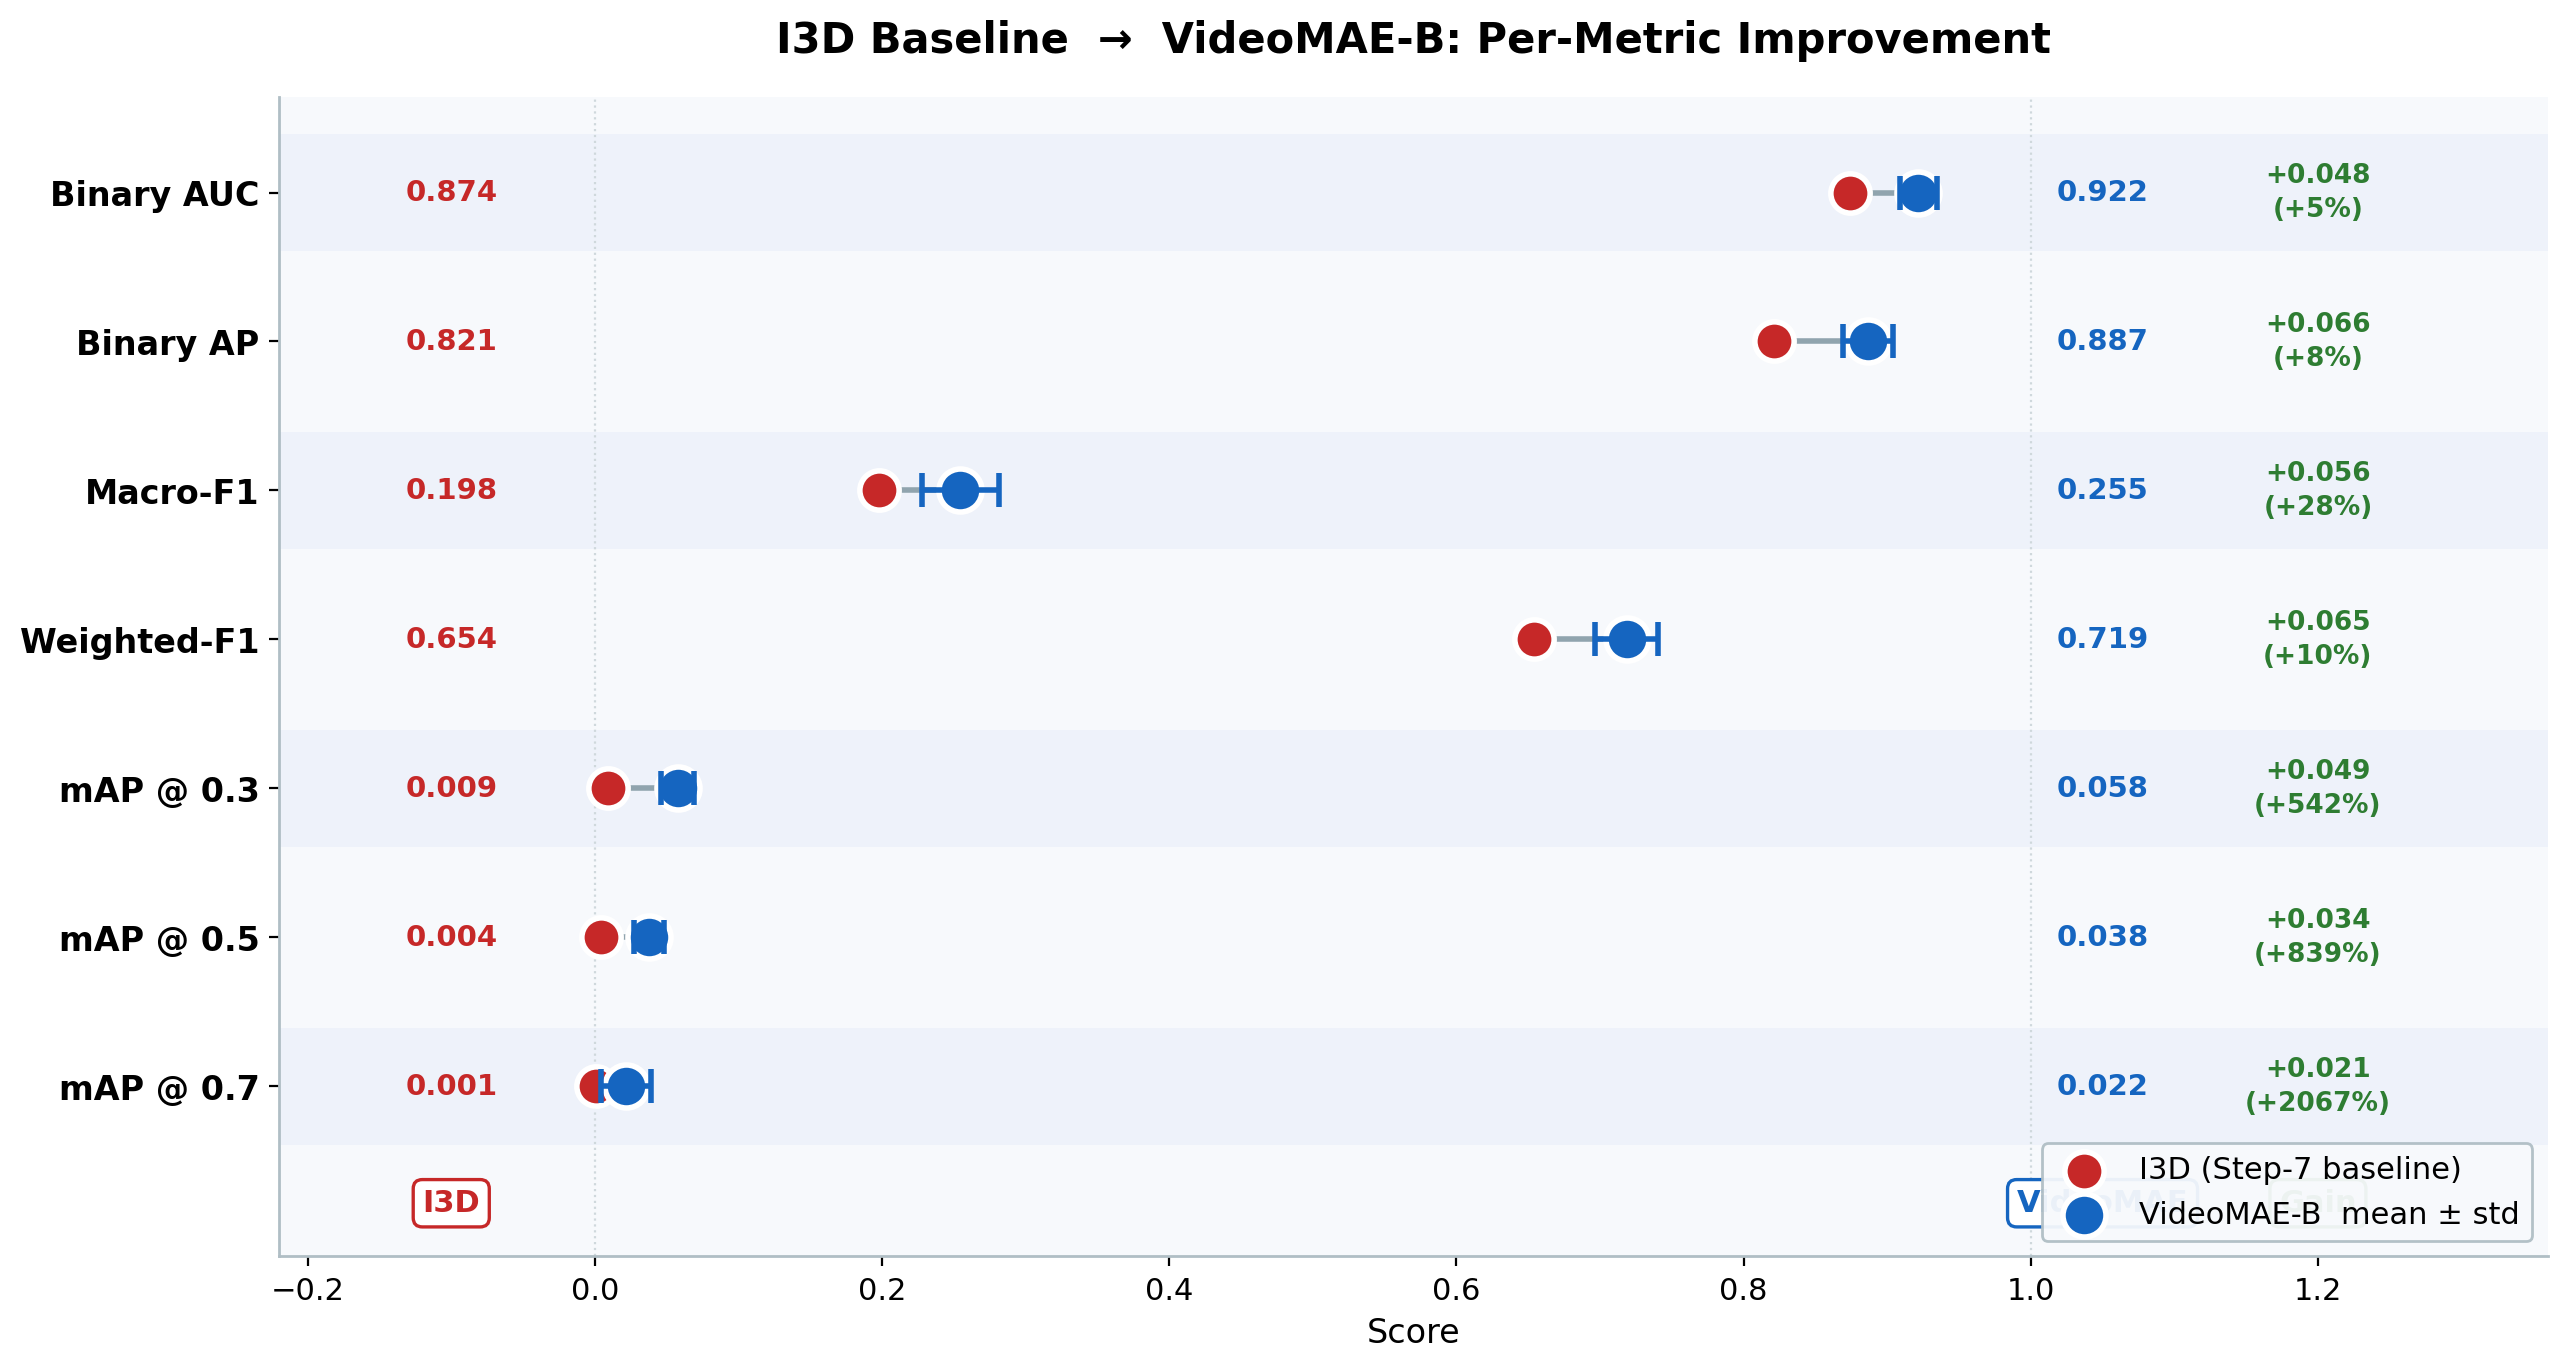
\includegraphics[width=\linewidth]{figures/fig2_dumbbell_comparison.png}
  \Description{Dumbbell chart comparing I3D and VideoMAE-B across seven
    metrics. Green gain badges show +4.8 pp AUC, +8\% AP, and up to
    x21.7 improvement in temporal mAP at IoU 0.7.}
  \caption{Per-metric improvement from I3D $\to$ VideoMAE-B (3-seed mean$\,\pm\,$std).
           Green badges show absolute gain and relative percentage.
           Localization metrics (mAP) improve by an order of magnitude.}
  \label{fig:dumbbell}
\end{figure}

\subsection{Full Detection Metrics}

Table~\ref{tab:full} reports all binary and multi-class metrics across three seeds.

\begin{table}[t]
  \centering
  \caption{Full evaluation metrics (VideoMAE-B, 3 seeds, UCF-Crime violence subset).}
  \label{tab:full}
  \small
  \begin{tabular}{l c c}
    \toprule
    \textbf{Metric}
      & \textbf{I3D baseline}
      & \textbf{VideoMAE-B (mean\,$\pm$\,std)} \\
    \midrule
    Binary AUC   & 0.874 & $0.922 \pm 0.013$ \\
    Binary AP    & 0.821 & $0.887 \pm 0.018$ \\
    Macro-F1     & 0.198 & $0.255 \pm 0.027$ \\
    Weighted-F1  & 0.654 & $0.719 \pm 0.022$ \\
    mAP@IoU\,0.3 & 0.009 & $0.058 \pm 0.012$ \\
    mAP@IoU\,0.5 & 0.004 & $0.038 \pm 0.008$ \\
    mAP@IoU\,0.7 & 0.001 & $0.022 \pm 0.010$ \\
    \bottomrule
  \end{tabular}
\end{table}

\subsection{Temporal Localization}

Figure~\ref{fig:map} plots mAP vs.\ tIoU threshold for both feature variants.
The VideoMAE-B advantage \emph{grows} with stricter overlap: ${\times}6.4$ at
IoU\,0.3 vs.\ ${\times}21.7$ at IoU\,0.7.
This suggests that VideoMAE features—trained with spatiotemporal masked
reconstruction—encode sharper temporal transitions than optical-flow-fused
I3D features, enabling the boundary head to predict more precise event
boundaries.

\begin{figure}[t]
  \centering
  
\includegraphics[width=\linewidth]{figures/fig3_localization_curve.png}
  \Description{Line chart of mAP versus tIoU threshold (0.3, 0.5, 0.7).
    VideoMAE-B (blue solid line) consistently exceeds I3D (red dashed line),
    with the gap widening at stricter thresholds.}
  \caption{mAP vs.\ tIoU threshold. VideoMAE-B (blue, solid) dominates
           I3D (red, dashed) at every threshold. The relative gain
           (${\times}6.4 \to {\times}9.4 \to {\times}21.7$) increases
           with stricter IoU, indicating sharper predicted boundaries.}
  \label{fig:map}
\end{figure}


%% ============================================================
\section{Analysis}
%% ============================================================

\subsection{Training Dynamics}

Figure~\ref{fig:training} shows training loss, validation AUC, and
validation Macro-F1 across 40 epochs for all three seeds.
Training loss converges smoothly by epoch 15.
AUC stabilises by epoch 10 at a high plateau ($>$0.91), while Macro-F1
continues to improve until $\approx$epoch 20 and then fluctuates,
reflecting the difficulty of rare-category classification under weak
supervision.
Cross-seed agreement is tight for AUC (std\,0.013) and somewhat looser
for Macro-F1 (std\,0.027), motivating future work on variance reduction
for multi-class heads.

\begin{figure*}[t]
  \centering
  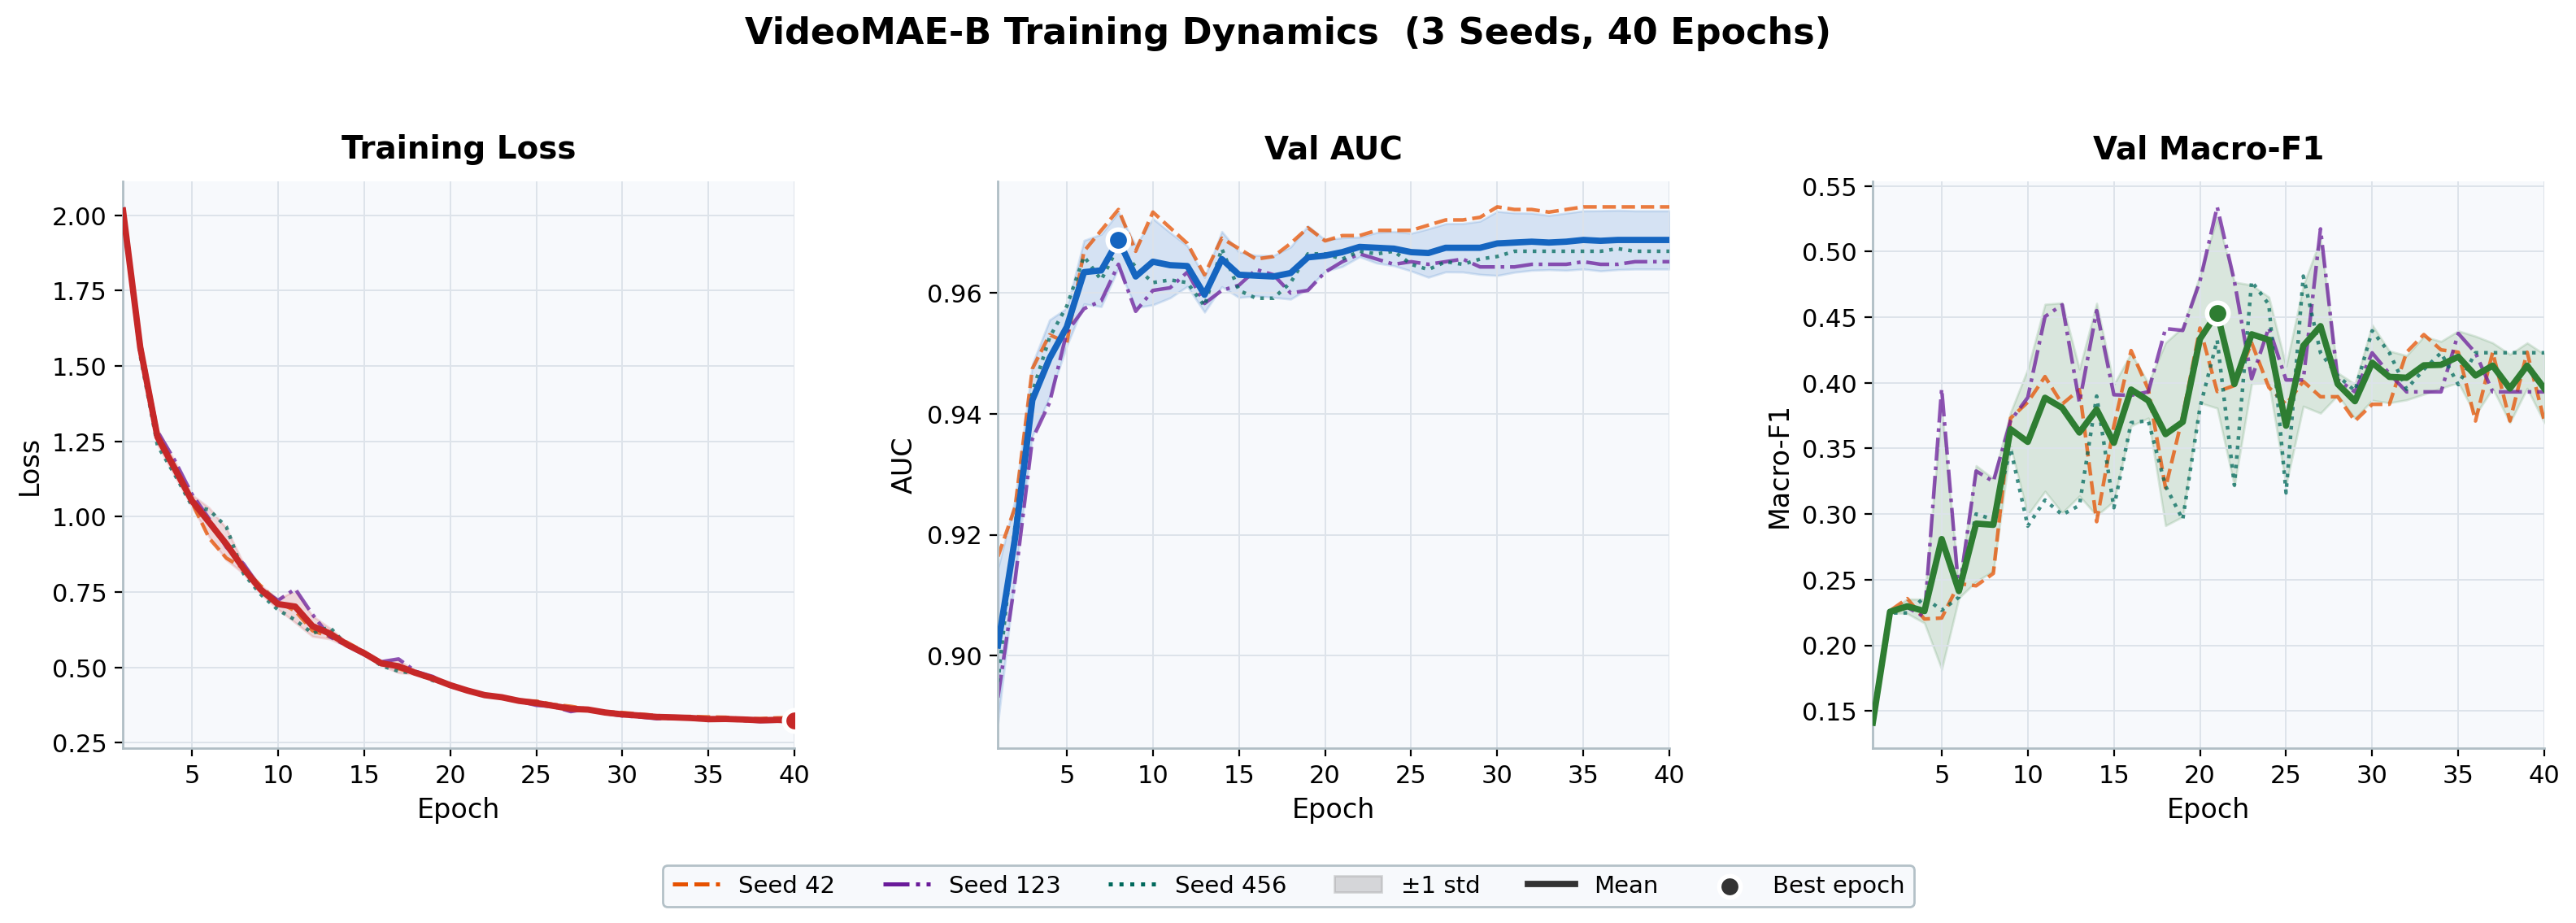
\includegraphics[width=\linewidth]{figures/fig1_training_dynamics.png}
  \Description{Three-panel plot of training dynamics over 40 epochs across
    three random seeds (mean and std band shown). Left: training loss converges
    smoothly by epoch~15. Center: validation AUC stabilises above 91\% from
    epoch~10. Right: validation Macro-F1 peaks near epoch~20.}
  \caption{Training dynamics over 40 epochs (3 seeds, mean\,$\pm$\,std band;
           dashed = individual seeds; dot = best epoch).
           \textbf{Left:} training loss---smooth convergence by epoch 15.
           \textbf{Center:} validation AUC---stable plateau above 91\% from epoch 10.
           \textbf{Right:} validation Macro-F1---peaks near epoch 20.}
  \label{fig:training}
\end{figure*}

\subsection{Cross-Seed Reproducibility}

Figure~\ref{fig:repro} plots per-seed values alongside the mean\,$\pm$\,std
for all six metrics.
Binary AUC varies only 1.26 pp across seeds (0.909--0.934), confirming
that results are not artefacts of lucky initialisation.
mAP metrics show higher but acceptable variance (${\pm}$1.2 at IoU\,0.3),
expected for temporally-sparse detections.

\begin{figure}[t]
  \centering
  
\includegraphics[width=\linewidth]{figures/fig4_reproducibility.png}
  \Description{Reproducibility plot showing per-seed metric values for
    three seeds alongside the mean and standard deviation. Binary AUC
    varies only 1.26 pp across seeds; mAP shows higher but acceptable
    variance.}
  \caption{Cross-seed reproducibility. Diamond ($\diamond$) = mean
           $\pm$\,1 std; circles = individual seeds.
           Binary metrics are highly stable; localization metrics show
           higher but acceptable variance.}
  \label{fig:repro}
\end{figure}

\subsection{Per-Class Analysis}

Figure~\ref{fig:perclass} compares per-category F1 between I3D and
VideoMAE-B for the best seed (seed\,123, AUC\,=\,0.934).
Key observations:
\begin{itemize}
  \item \textbf{Explosion} benefits most ($+$0.24), from F1\,0.18 to 0.41.
        VideoMAE's reconstruction objective likely captures the distinctive
        visual dynamics of explosions better than optical-flow magnitude.
  \item \textbf{Normal class} improves from 0.81 to 0.92 ($+$0.11),
        confirming better discrimination of non-anomalous footage.
  \item \textbf{Shooting} and \textbf{Robbery} regress slightly
        ($-$0.11 and $-$0.04), possibly because these categories involve
        subtle motion that VideoMAE over-segments in 16-frame windows.
  \item \textbf{Fighting} collapses to F1\,=\,0.00 despite the overall
        macro improvement. Fighting shares motion statistics with normal
        crowded scenes; 16-frame context appears insufficient to discriminate
        the build-up dynamics.
\end{itemize}

\begin{figure}[t]
  \centering
  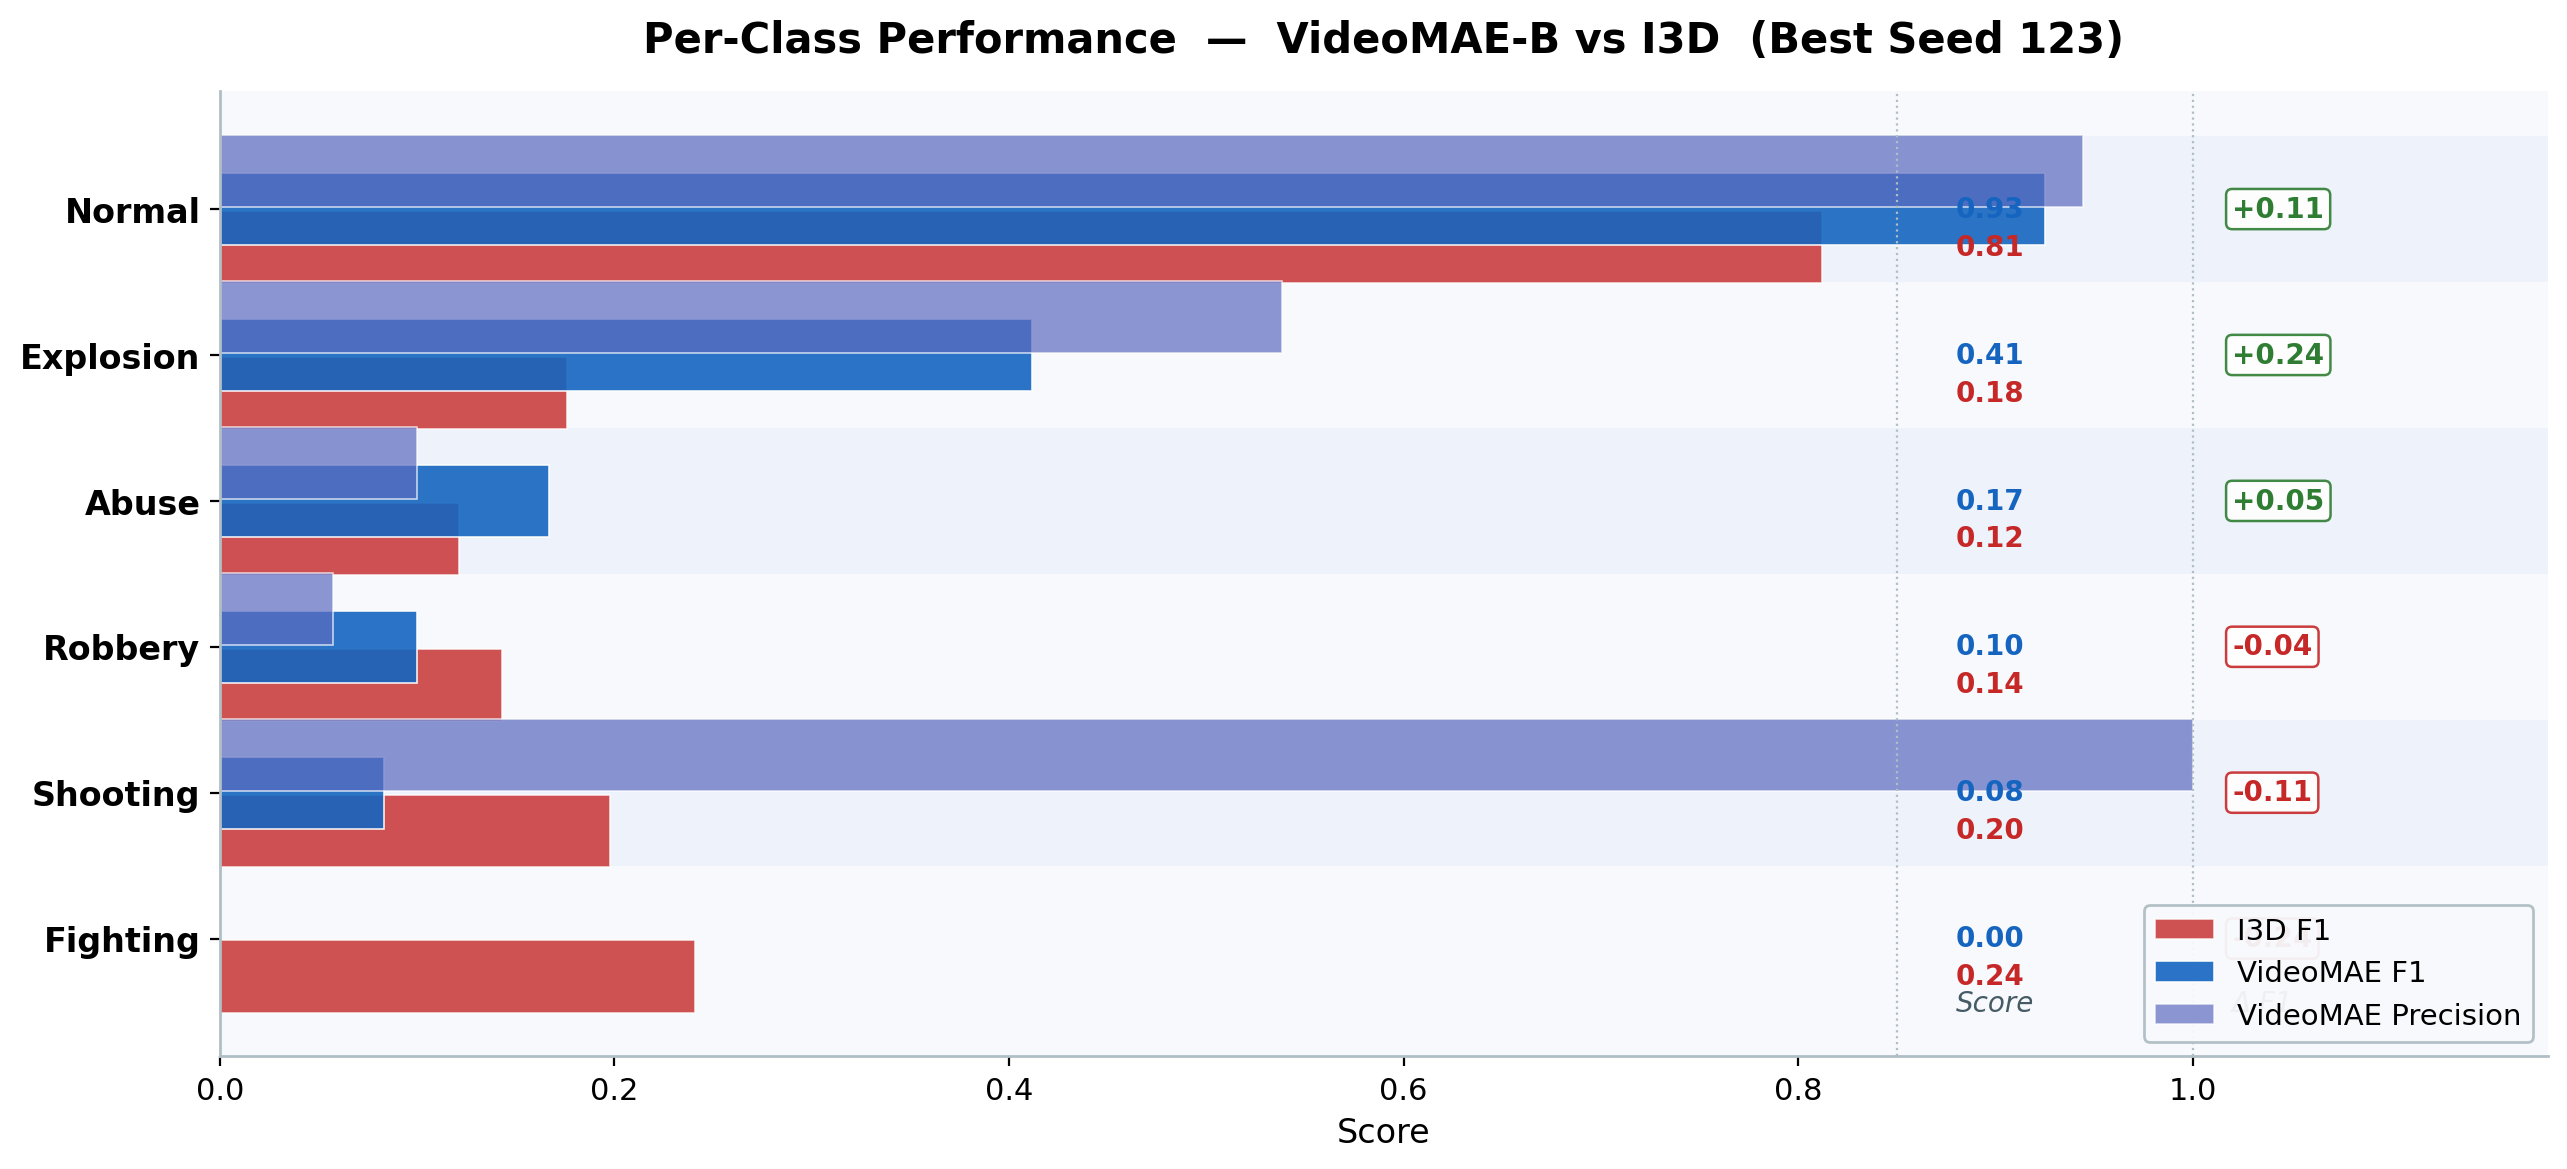
\includegraphics[width=\linewidth]{figures/fig5_per_class.png}
  \Description{Grouped bar chart showing per-class F1 for I3D (red) and
    VideoMAE-B (blue) across six categories. Explosion improves most
    (+0.24 F1). Fighting collapses to 0 for VideoMAE-B. Delta badges on
    the right indicate gain or regression relative to I3D.}
  \caption{Per-class F1---I3D (red) vs.\ VideoMAE-B (blue), best seed 123.
           Purple bars show VideoMAE-B precision.
           Delta badges (far right) show gain (green) or
           regression (red) vs.\ I3D.}
  \label{fig:perclass}
\end{figure}

\subsection{All-Metrics Overview}

Figure~\ref{fig:radar} shows a radar chart summarising all five metrics
across both models (3-seed mean).
VideoMAE-B strictly dominates I3D on the radar on every axis, with the
largest angular gap at AP and AUC and a visually striking improvement
at the mAP vertices.

\begin{figure}[t]
  \centering
  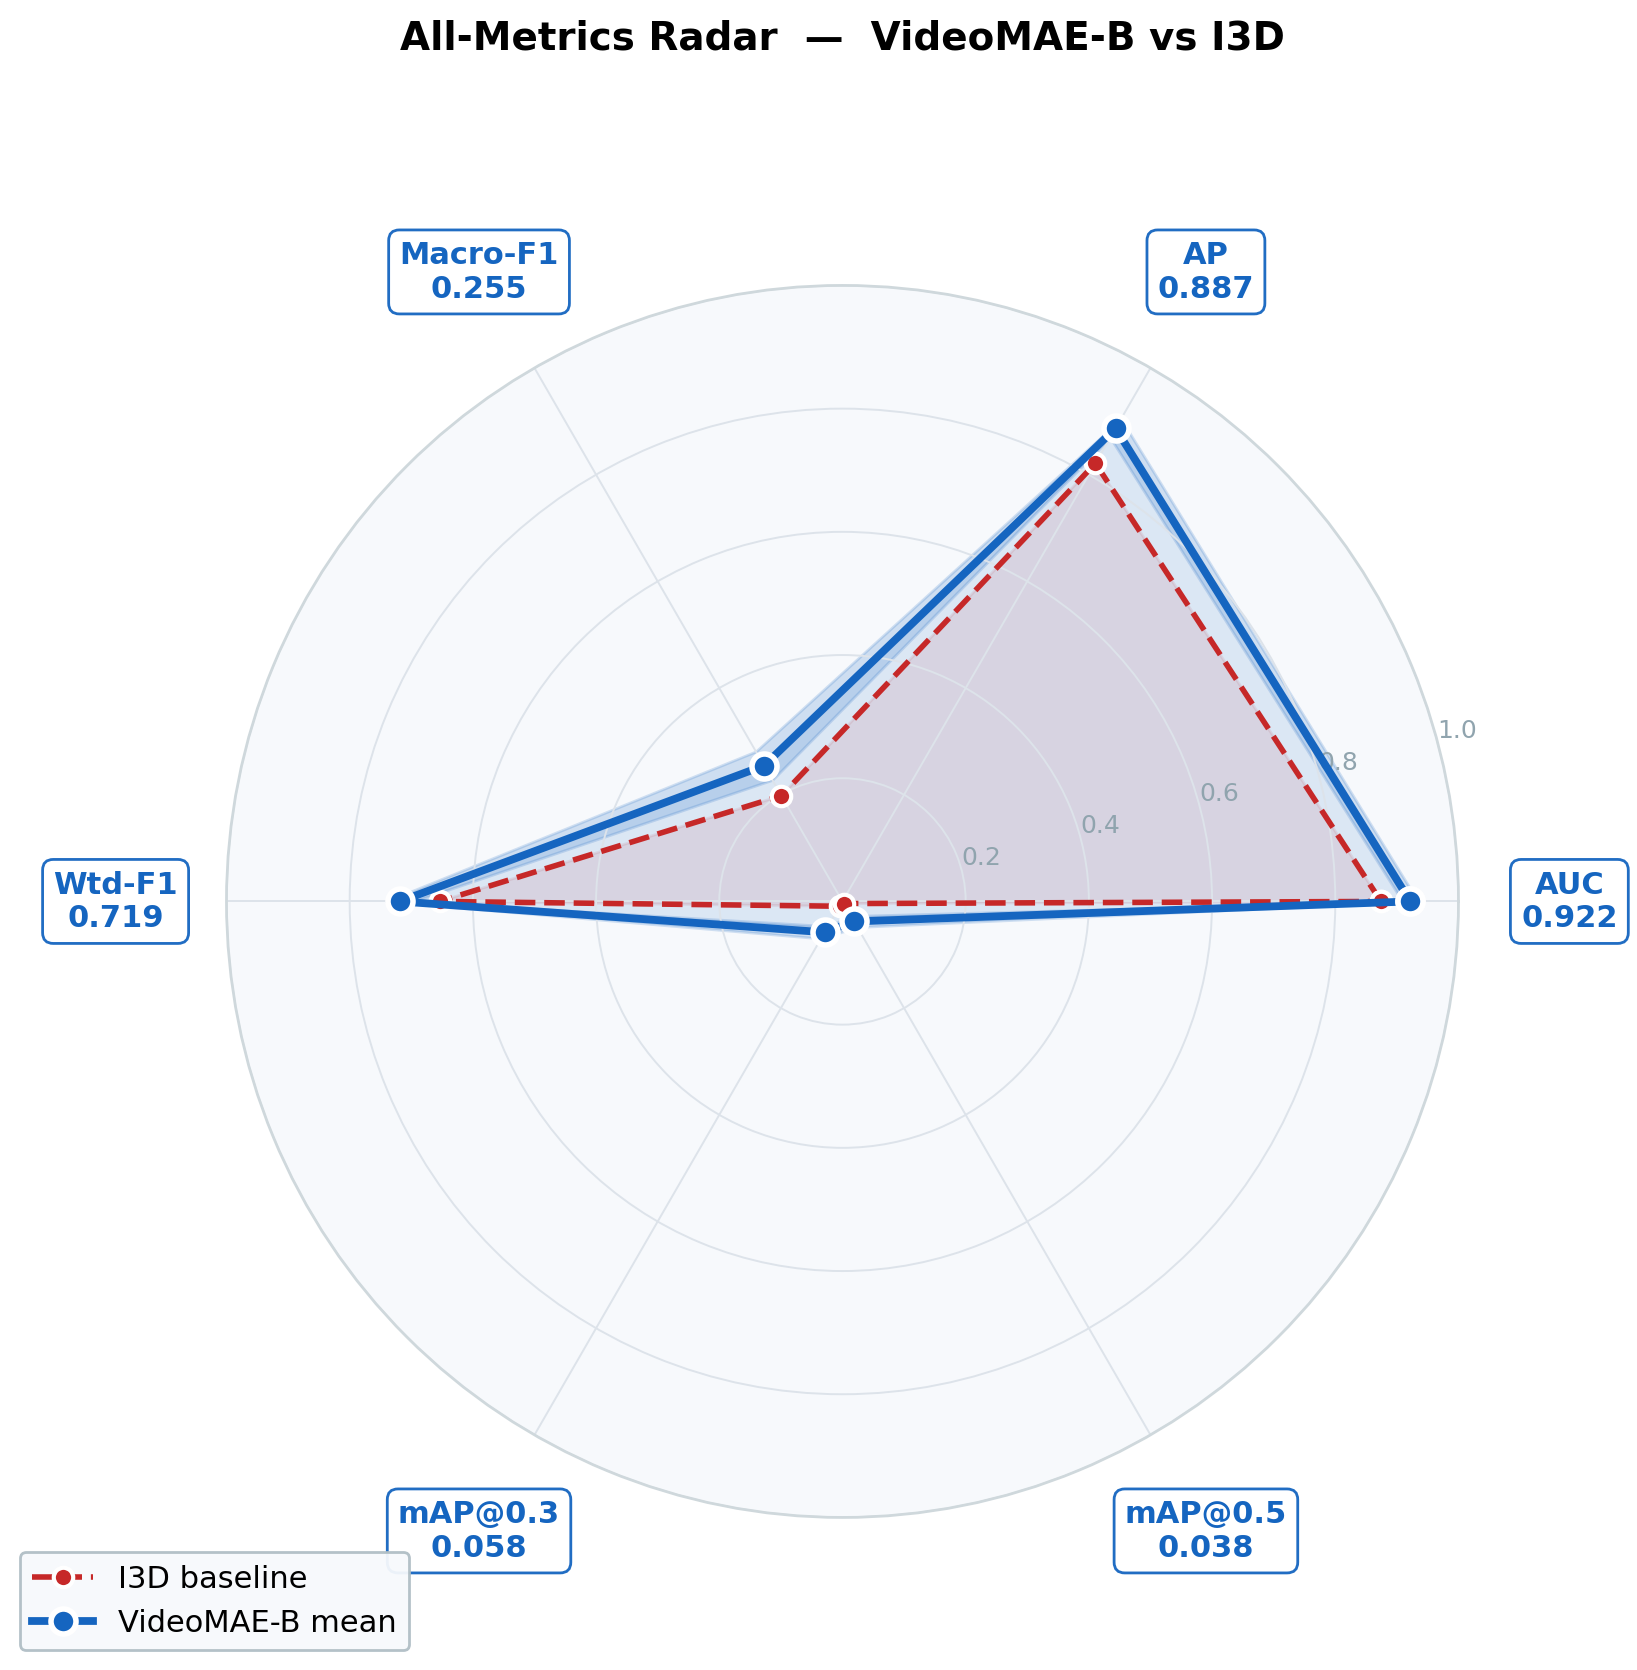
\includegraphics[width=0.88\linewidth]{figures/fig6_radar_overview.png}
  \Description{Radar chart with five axes (AUC, AP, Macro-F1, mAP@0.3,
    mAP@0.7). VideoMAE-B (blue filled polygon) encloses the I3D baseline
    (red dashed polygon) on every axis, with the largest gap at mAP
    vertices.}
  \caption{All-metrics radar---VideoMAE-B (blue, 3-seed mean) vs.\
           I3D baseline (red dashed). VideoMAE-B dominates every axis.}
  \label{fig:radar}
\end{figure}

\subsection{Discussion}
\label{sec:discuss}

\paragraph{Comparison caveat.}
Published SOTA rows in Table~\ref{tab:main} use frame-level AUC evaluated
on all 13 anomaly categories of UCF-Crime, while our rows use the 6-category
violence subset with video-level AUC.
These evaluations are \emph{not} directly comparable; we include published
numbers only to situate our work in the broader landscape.
Within our controlled I3D-vs-VideoMAE-B comparison, the backbone swap
yields $+$4.8\,pp AUC and ${\times}6.4$ mAP@0.3—a strong signal
regardless of evaluation differences.

\paragraph{Why localization improves most.}
VideoMAE's reconstruction pre-training forces the model to reason about
spatiotemporal continuity across masked patches, producing features that
encode temporal transitions more precisely than I3D's optical-flow stream.
This directly benefits the boundary head, explaining the disproportionate
mAP gain at strict IoU thresholds.

\paragraph{Failure cases.}
The Fighting class collapse and the gap between Macro-F1 (0.255) and
Weighted-F1 (0.719) reveal that rare categories remain challenging.
16-frame windows appear too short for fight build-up dynamics; longer
context windows or hierarchical aggregation are natural remedies.


%% ============================================================
\section{Conclusion}
%% ============================================================

We demonstrated that replacing frozen I3D features with frozen VideoMAE-B
features in a weakly-supervised RTFM + TRN + Boundary Head pipeline yields
consistent, large improvements in violence detection and temporal localization
on the UCF-Crime violence subset.
Improvements are largest for temporal localization (up to ${\times}21.7$
mAP gain at strict IoU thresholds), suggesting that VideoMAE's
masked-autoencoding pre-training encodes sharper event boundaries than
I3D's optical-flow-based representations.
A lightweight training recipe—inverse-frequency class weights,
confidence-thresholded pseudo-labels, and cosine annealing LR—further
stabilises results across seeds.

\paragraph{Limitations and future work.}
Macro-F1 remains low (25.5\%), driven primarily by the Fighting class
collapse under 16-frame segmentation.
Future directions include: (i)~cross-dataset evaluation on XD-Violence
and ShanghaiTech, (ii)~longer-context windows (32 or 64 frames),
(iii)~VideoMAE-Large backbone, and (iv)~semi-supervised fine-tuning when
sparse frame-level annotations are available.


%% ============================================================
%% References  (inline — no .bib file needed in Overleaf)
%% ============================================================
\begin{thebibliography}{16}

\bibitem{sultani2018real}
W.~Sultani, C.~Chen, and M.~Shah.
\newblock Real-world anomaly detection in surveillance videos.
\newblock In \emph{CVPR}, pages 6479--6488, 2018.

\bibitem{tian2021weakly}
Y.~Tian, G.~Pang, Y.~Chen, R.~Singh, J.~W. Verjans, and G.~Carneiro.
\newblock Weakly-supervised video anomaly detection with robust temporal
  feature magnitude learning.
\newblock In \emph{ICCV}, pages 4975--4986, 2021.

\bibitem{tong2022videomae}
Z.~Tong, Y.~Song, J.~Wang, and L.~Wang.
\newblock {VideoMAE}: Masked autoencoders are data-efficient learners for
  self-supervised video pre-training.
\newblock In \emph{NeurIPS}, volume~35, pages 10078--10093, 2022.

\bibitem{carreira2017quo}
J.~Carreira and A.~Zisserman.
\newblock Quo vadis, action recognition? {A} new model and the kinetics
  dataset.
\newblock In \emph{CVPR}, pages 6299--6308, 2017.

\bibitem{chen2023mgfn}
M.~Chen, R.~Zeng, J.~Jiao, and T.~Liu.
\newblock {MGFN}: Magnitude-contrastive glance-and-focus network for
  weakly-supervised video anomaly detection.
\newblock In \emph{AAAI}, volume~37, pages 387--395, 2023.

\bibitem{wu2024vadclip}
P.~Wu, X.~Zhou, G.~Pang, L.~Zhou, Q.~Yan, P.~Wang, and Y.~Zhang.
\newblock {VadCLIP}: Adapting vision-language models for weakly supervised
  video anomaly detection.
\newblock In \emph{AAAI}, 2024.

\bibitem{wu2020not}
P.~Wu, J.~Liu, Y.~Shi, Y.~Sun, F.~Shao, Z.~Wu, and Z.~Yang.
\newblock Not only look, but also listen: Learning multimodal violence
  detection under weak supervision.
\newblock In \emph{ECCV}, pages 322--339, 2020.

\bibitem{zhang2022actionformer}
C.-L. Zhang, J.~Wu, and Y.~Li.
\newblock {ActionFormer}: Localizing moments of actions with transformers.
\newblock In \emph{ECCV}, pages 492--510, 2022.

\bibitem{shi2023tridet}
D.~Shi, Y.~Zhong, Q.~Cao, L.~Ma, J.~Li, and D.~Tao.
\newblock {TriDet}: Temporal action detection with relative boundary modeling.
\newblock In \emph{CVPR}, pages 18857--18866, 2023.

\bibitem{wu2023surveillance}
J.~Wu, W.~Zhang, G.~Li, W.~Wu, X.~Tan, Y.~Li, E.~Ding, and L.~Lin.
\newblock Weakly supervised video anomaly detection via self-guided temporal
  discriminative transformer.
\newblock \emph{IEEE TCSVT}, 33(10):6216--6228, 2023.

\bibitem{lan2025dss}
S.~Lan, X.~Wang, Y.~Song, Y.~Zhan, G.~Zhang, and C.-W. Lin.
\newblock Weakly supervised video anomaly detection with discriminative score
  suppression and temporal refinement.
\newblock In \emph{WACV}, pages 1740--1750, 2025.

\bibitem{wang2025dakd}
X.~Wang, S.~Lan, Y.~Song, Y.~Zhan, and C.-W. Lin.
\newblock Weakly supervised video anomaly detection with distilled attention
  and knowledge distillation.
\newblock In \emph{WACV}, pages 1710--1719, 2025.

\bibitem{tian2025lecvad}
Y.~Wang and S.~Chen.
\newblock Learning event completeness for weakly supervised video anomaly
  detection.
\newblock In \emph{ICML}, 2025.

\bibitem{wang2025gsmoe}
X.~Wang, Y.~Wang, S.~Wei, and Q.~Zhang.
\newblock {GS-MoE}: Category-specific supervision and generation mechanism
  based sparse mixture of experts for weakly supervised video anomaly
  detection.
\newblock In \emph{ICCV}, pages 31628--31639, 2025.

\bibitem{wang2022internvideo}
Y.~Wang, K.~Li, Y.~Li, Y.~He, B.~Huang, et~al.
\newblock {InternVideo}: General video foundation models via generative and
  discriminative learning.
\newblock \emph{arXiv:2212.03191}, 2022.

\bibitem{maaz2023videochatgpt}
M.~Maaz, H.~Rasheed, S.~Khan, and F.~S. Khan.
\newblock {Video-ChatGPT}: Towards detailed video understanding via large
  vision and language models.
\newblock In \emph{ACL}, pages 14410--14425, 2024.

\end{thebibliography}

\end{document}
